% \cleardoublepage
\chapter{Requirement Analysis}\label{sec:reqs}\minitoc\vspace{.5cm}
\index{Requirements}

\section{Introduction}
The objective of this project is to conduct research and implement the concept of a multipath networking tunnel utilizing the \ac{xdppage} technology. The project aims to deliver a comprehensive thesis documentation along with a functional implementation, preferably in the form of a test program based on the \ac{MTX} tunnel designed as a programming library.
This \ac{MTX} library will enable the establishment of a network tunnel between two machines, allowing traffic to flow simultaneously over multiple network links. 
The test program will serve as a demonstration platform for the library, simulating a transport session using the \ac{gptu} protocol — a 5G technology employed for tunneling a significant volume of non-homogeneous data.
During the demonstration, the library's capabilities will be showcased, including flow management, throughput control, and other essential features that align with the intended purpose of the library.

\section{Current solution}
% Multipath is equivalent to horizontal scaling to increase connection capacity.
% It is also a method to achieve better reliability by building redundancy.
% Quality of service can also be improve by providing treatment and links optimized for different data flows.
% By establishing a multipath tunnel, the resources of each path can be monitored and scheduled between concurrent applications and leads to better utilization and efficiency.
Multipath technique serves as a means of horizontally scaling networking capacity by aggregating resources to increase connection bandwidth. 
Additionally, it offers a way to enhance reliability by incorporating redundancy into the network connection. Furthermore, multipath can improve quality of service by enabling optimized treatment and dedicated links for different types of data flows.
Finally, through the establishment of a multipath tunnel, the resources available on each path can be monitored and efficiently allocated among concurrent applications. 
This leads to improved resource utilization and overall efficiency in the network.

Current tunnel and VPN solutions available in the market are limited to single-path functionality. While protocols like \ac{MPTCP} and \ac{SCTP} are well-known for their multipath capabilities, they are primarily designed for exclusive use by a single caller.
Our focus lies in exploring how high-demand applications, particularly within the 5G infrastructure, handle the substantial traffic volume. Interestingly, certain implementations leverage DPDK to enhance packet forwarding and processing capabilities beyond the limitations of the Linux network stack. However, these software stacks are not readily accessible for research and testing purposes without purchasing expensive system.

\section{Proposed solution}
To address the need for a multipath connection that supports non-homogeneous and concurrent usage, we introduce the concept of a multipath tunnel. 
Our proposal aims to bridge the gap by enabling the utilization of multiple paths simultaneously.
To ensure optimal path utilization and minimal latency, we will utilize \ac{xdppage} technology to handle the movement of tunnel traffic. 
Specifically, the tunnel traffic will consist of UDP packets, allowing for efficient and effective data transmission.
The following section will present the requirements for the project \todo{improve}.

\subsection{Functional requirements}
% Functional requirements describes the high-level functionality of the system.
We define the functional requirements for the \ac{MTX} library:
\begin{itemize}
    \item Given multiple \ac{NIC}s, \ac{MTX} library shall be able to establish a tunnel between 2 hosts and exchange data through the tunnel over the chosen \ac{NIC}s.
    \item The \ac{MTX} library shall send and receive tunnel's UDP packets using \ac{xdppage} socket exclusively.
    \item The\ac{MTX} library shall support for path-level control and treatment, including scheduling, path failure detection and initiation. \todo{more}
    \item The\ac{MTX} library shall provide support for flow-level control and treatment, including setting and enforcing priority, traffic shaping, resource allocation for sensitive requirement (i.e path for low latency data).
    \item A centralized controller shall be provided. Users shall have access to configuration options for the aforementioned features.
\end{itemize}

\subsection{Nonfunctional requirements}
We define the non-functional requirements for the \ac{MTX} library:
\begin{itemize}
    \item Usability: \ac{MTX} library should be used similar to a Linux socket. A global configuration will be responsible for managing the overall configuration of the tunnel. On the other hand, each caller will have the ability to configure the traffic characteristics according to their specific requirements.
    \item Performance and Reliability: The tunnel is expected to deliver throughput asymptotic to the line rate while having very low negative effect on overall system load thanks to \ac{xdppage} technology. Measuring is rather complicated since the code quality can't be ensured and high performance hardware will be needed. This problem should be addressed in the course of the project.
\end{itemize}

\subsection{System models}
Intended to be a general purpose multipath tunnel, \ac{MTX} is designed to be the wrapper around transport layer to abstract the multipath details.
Callers interact with the tunnel through shared memory or a TUN\TAP interface. This will be discussed further.
The library can be considered for application where reliability, high performance and ease of maintain requirements converge \todo{more}.

% \begin{wrapfigure}{r}{0.2\textwidth}
%     \centering
%     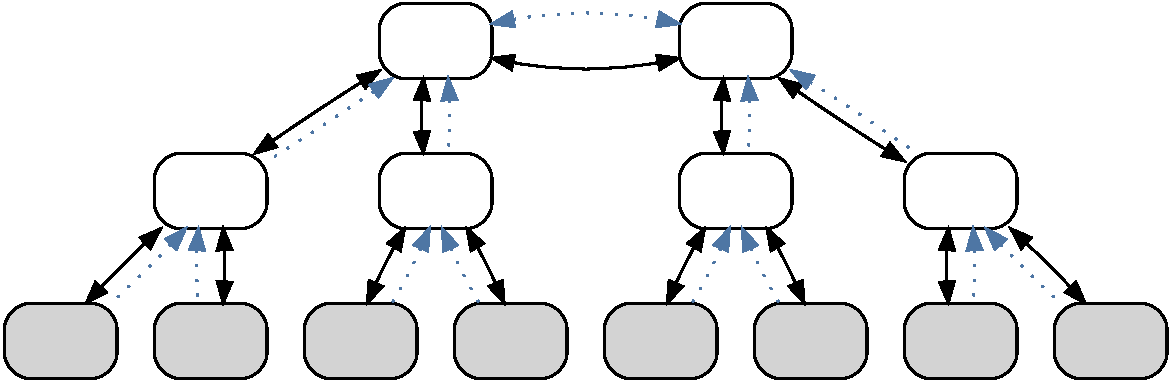
\includegraphics[width=0.2\textwidth]{resources/images/example3}
% \end{wrapfigure}

% \sidenote{Overview}
% \todomid{write about \Cref{fig:req:details}}

% \begin{figure}[H]
%     \centering
%     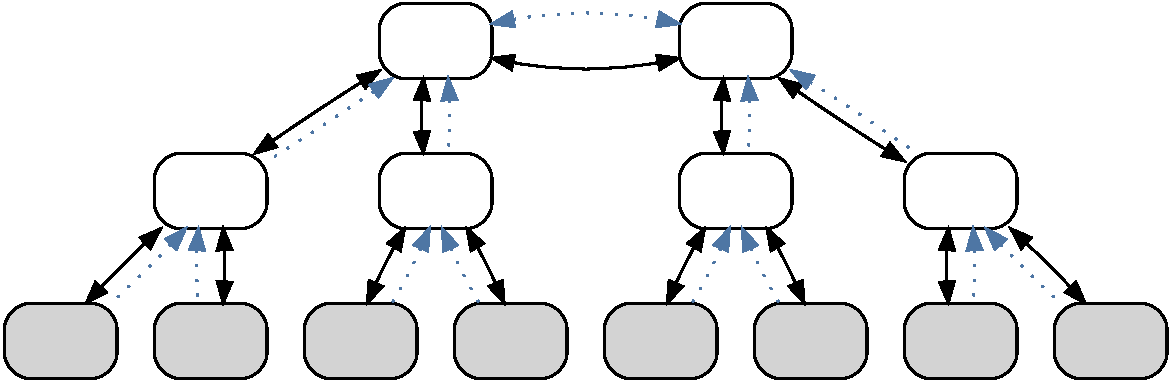
\includegraphics[width=.85\textwidth]{resources/images/example3}
%     \caption{More detailed overview of the requirements}\label{fig:req:details}
% \end{figure}

% \sidenote{Structure of Research}
% \todomid{write about \Cref{fig:hourglass:reqs}}

% \begin{figure}[H]
%     \centering
%     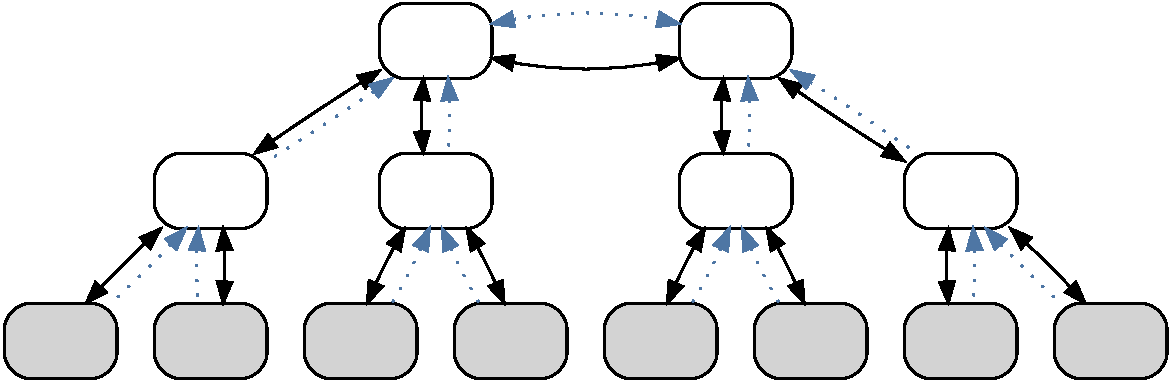
\includegraphics[width=.55\textwidth]{resources/images/example3}
%     \caption{Placement of the requirement section in the structure of research}\label{fig:hourglass:reqs}
% \end{figure}

% \section{Stakeholder 1}

% \sidenote{\Cref{tbl:reqs:stakeholder1}}
% \todomid{write about \Cref{tbl:reqs:stakeholder1}}

% \begin{tabularx}{\textwidth}{lX}
%     \caption{Requirements from stakeholder 1 perspective}\label{tbl:reqs:stakeholder1}\\
%     \toprule
%     \textbf{\#}& \textbf{Description}  \\\midrule
%     \endfirsthead%
%     \toprule
%     \textbf{\#}& \textbf{Description}  \\\midrule
%     \endhead%
%     \requirement{U}{req:stakeholder1:foo}{Foo}
%        & \todomid{write}
%     \\\midrule
%     \requirement{U}{req:stakeholder1:bar}{Bar}
%        & \todomid{write}
%     \\\bottomrule
% \end{tabularx}

% \section{Stakeholder 2}

% \sidenote{\Cref{tbl:reqs:stakeholder2}}
% \todomid{write about \Cref{tbl:reqs:stakeholder2}}

% \begin{tabularx}{\textwidth}{lX}
%     \caption{Requirements from stakeholder 2 perspective}\label{tbl:reqs:stakeholder2}\\
%     \toprule
%     \textbf{\#}& \textbf{Description}  \\\midrule
%     \endfirsthead%
%     \toprule
%     \textbf{\#}& \textbf{Description}  \\\midrule
%     \endhead%
%     \requirement{S}{req:stakeholder2:foo}{Foo}
%        & \todomid{write}
%     \\\midrule
%     \requirement{S}{req:stakeholder2:bar}{Bar}
%        & \todomid{write}
%     \\\bottomrule
% \end{tabularx}

% \section{Stakeholder 3}

% \sidenote{\Cref{tbl:reqs:stakeholder3}}
% \todomid{write about \Cref{tbl:reqs:stakeholder3}}

% \begin{tabularx}{\textwidth}{lX}
%     \caption{Requirements from stakeholder 3 perspective}\label{tbl:reqs:stakeholder3}\\
%     \toprule
%     \textbf{\#}& \textbf{Description}  \\\midrule
%     \endfirsthead%
%     \toprule
%     \textbf{\#}& \textbf{Description}  \\\midrule
%     \endhead%
%     \requirement{T}{req:stakeholder3:foo}{Foo}
%        & \todomid{write}
%     \\\midrule
%     \requirement{T}{req:stakeholder3:bar}{Bar}
%        & \todomid{write}
%     \\\bottomrule
% \end{tabularx}

% \section{Conclusion}

% \sidenote{Summary}
% \todomid{write}

% \sidenote{Takeaway 1}
% \todomid{write}

% \sidenote{Takeaway 2}
% \todomid{write}

% \sidenote{Takeaway 3}
% \todomid{write}

% \sidenote{Next chapter}
% \todomid{write}